\documentclass[9pt,dvipsnames]{beamer}
\usepackage[T1]{fontenc}
\usepackage{libertinus}
\usepackage{amsmath}
\usepackage[most]{tcolorbox}

\usepackage{graphicx}
\usepackage{booktabs}
\usepackage{hyperref}
\hypersetup{
	colorlinks=true, % Enable coloring of links
	% urlcolor=blue    % Set the color of URL links to blue
}

\usepackage{xcolor}  
\newcommand{\cb}[1]{{\color{CadetBlue}#1}}


\usetheme{Berkeley}
\setbeamertemplate{navigation symbols}{}


\title{CSE574 Introduction to Machine Learning}
\subtitle{Machine Learning: Fundamental Algorithms Part 2}
\author{Jue Guo}
\institute{University at Buffalo}
\date{\today}

\begin{document}
	\begin{frame}
		\titlepage
	\end{frame}
	
	\begin{frame}
		\frametitle{Outline}
		\tableofcontents
	\end{frame}
	\section{Decision Tree Learning}
	\begin{frame}{Decision Tree Learning}
		A \textbf{decision tree} is an \textbf{acyclic} graph that can be used to make decisions. 
		\begin{itemize}
			\item In each branching node of the graph, a specific feature $j$ of the feature vector is examined. If the value of the feature is below a specific threshold, then the left branch is followed; otherwise, the right branch is followed. 
			\item As the leaf node is reached, the decision is made about the class to which the example belongs.
		\end{itemize}
	\end{frame}
	\subsection{Problem Statement}
	\begin{frame}{Problem Statement}
		Like previously, we have a collection of labeled examples; labels belong to the set $\{0,1\}$. We want to build a decision tree that would allow us to predict the class given a feature vector.
	\end{frame}
	\subsection{Solution}
	\begin{frame}{Solution}
		There are various formulations of the decision tree learning algorithm: 
		\begin{itemize}
			\item Iterative Dichotomiser 3 (\textbf{ID3})
			\item \textbf{C4.5} (Written in C and 4.5 is just the version name)
		\end{itemize}
	\end{frame}
	\subsubsection{ID3}
	\begin{frame}{ID3}
		First, the \textcolor{red}{ID3}. 
		The optimization criterion, in this case, is the average log-likelihood:
		
		$$
		\frac{1}{N} \sum_{i=1}^{N}\left[y_{i} \ln f_{I D 3}\left(\mathbf{x}_{i}\right)+\left(1-y_{i}\right) \ln \left(1-f_{I D 3}\left(\mathbf{x}_{i}\right)\right)\right]
		$$
		
		where $f_{I D 3}$ is a decision tree.
		
		By now, it looks very similar to logistic regression. 
		\begin{itemize}
			\item However, contrary to the logistic regression learning algorithm which builds a \textbf{parametric model} $f_{\mathrm{w}^{*}, b^{*}}$ by finding an optimal solution to the optimization criterion, the ID3 algorithm optimizes it approximately by constructing a \textbf{nonparametric model} $f_{I D 3}(\mathbf{x}) \stackrel{\text { def }}{=} \operatorname{Pr}(y=1 \mid \mathbf{x})$.
		\end{itemize}
	\end{frame}
	
	\begin{frame}
		\begin{figure}
			\centering
			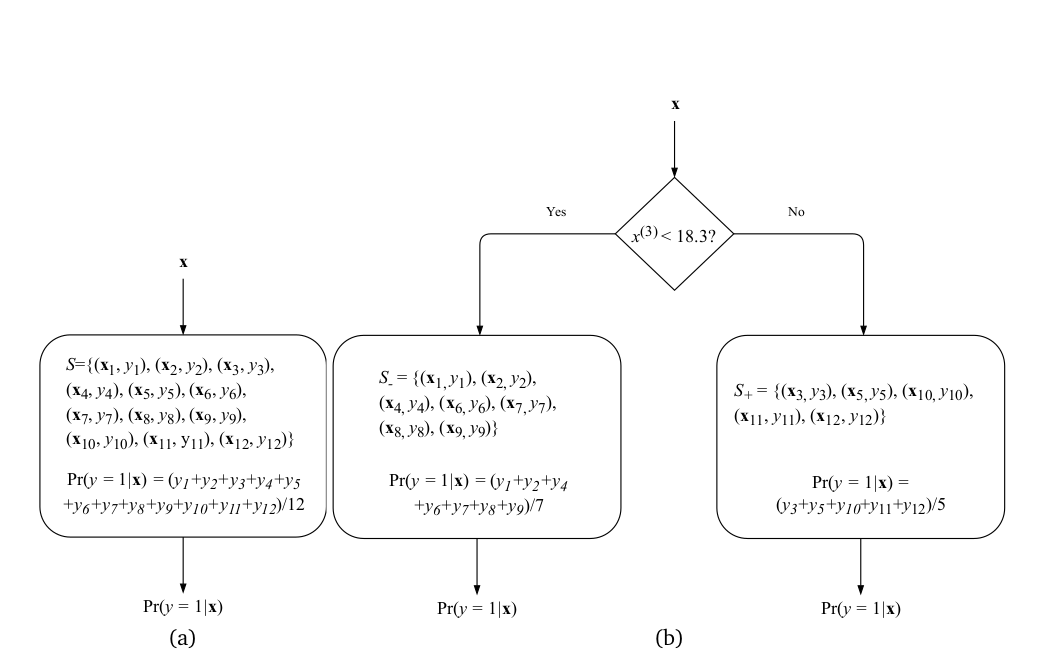
\includegraphics[width=0.7\textwidth]{imgs/algorithm_4.png}
			\caption{An illustration of a decision tree building algorithm. The set $\mathcal{S}$ contains 12 labeled examples. (a) In the beginning, the decision tree only contains the start node; it makes the same prediction for any input. (b) The decision tree after the first split; it tests whether feature 3 is less than 18.3 and, depending on the result, the prediction is made in one of the two leaf nodes.}
		\end{figure}
	\end{frame}
	
	\begin{frame}
		The ID3 learning algorithm works as follows. Let $\mathcal{S}$ denote a set of labeled examples. \textbf{In the beginning}, the decision tree only has a start node that contains all examples: $\mathcal{S} \stackrel{\text { def }}{=}$ $\left\{\left(\mathbf{x}_{i}, y_{i}\right)\right\}_{i=1}^{N}$. Start with a constant model $f_{I D 3}^{S}$ defined as,
		
		$$
		f_{I D 3}^{\mathcal{S}} \stackrel{\text { def }}{=} \frac{1}{|\mathcal{S}|} \sum_{(\mathbf{x}, y) \in \mathcal{S}} y
		$$
		
		The prediction given by the above model, $f_{I D 3}^{S}(\mathbf{x})$, would be the same for any input $\mathbf{x}$. The corresponding decision tree built using a toy dataset of 12 labeled examples is shown in left of the figure.
	\end{frame}
	
	\begin{frame}
		\textbf{Then} we search through all features $j=1, \ldots, D$ and all thresholds $t$, and split the set $S$ into two subsets: $\mathcal{S}_{-} \stackrel{\text { def }}{=}\left\{(\mathbf{x}, y) \mid(\mathbf{x}, y) \in \mathcal{S}, x^{(j)}<t\right\}$ and $\mathcal{S}_{+} \stackrel{\text { def }}{=}\left\{(\mathbf{x}, y) \mid(\mathbf{x}, y) \in S, x^{(j)} \geq t\right\}$. 
		\begin{itemize}
			\item The two new subsets would go to two new leaf nodes, and we evaluate, for all possible pairs $(j, t)$ how good the split with pieces $\mathcal{S}_{-}$and $\mathcal{S}_{+}$is.
		\end{itemize}
		 \textbf{Finally}, we pick the best such values $(j, t)$, split $\mathcal{S}$ into $\mathcal{S}_{+}$and $\mathcal{S}_{-}$, form two new leaf nodes, and continue recursively on $\mathcal{S}_{+}$and $\mathcal{S}_{-}$(\textit{or quit if no split produces a model that's sufficiently better than the current one}).
	\end{frame}
	
	\begin{frame}{``How good the split is?"}
		Now you should wonder what do the words "evaluate how good the split is" mean. In ID3, the goodness of a split is estimated by using the criterion called \textbf{entropy}.
		\begin{itemize}
			\item Entropy is a measure of uncertainty about a random variable. It reaches its maximum when all values of the random variables are equiprobable. Entropy reaches its minimum when the random variable can have only one value.
		\end{itemize}
		 The entropy of a set of examples $\mathcal{S}$ is given by,
		
		$$
		H(\mathcal{S}) \stackrel{\text { def }}{=}-f_{I D 3}^{\mathcal{S}} \ln f_{I D 3}^{\mathcal{S}}-\left(1-f_{I D 3}^{\mathcal{S}}\right) \ln \left(1-f_{I D 3}^{\mathcal{S}}\right)
		$$
		\begin{itemize}
			\item \(f_{I D 3}^{\mathcal{S}}\) is the probability of an example in $\mathcal{S}$ being of a particular class.
			\item \textbf{Maximum Entropy}: When the classes are evenly split (i.e., $f_{I D 3}^{\mathcal{S}}=0.5$ in a binary classification), entropy reaches its maximum, indicating maximum uncertainty or disorder. In this case, predicting the class of a new sample is as uncertain as a coin flip.
			\item \textbf{Minimum Entropy}: When all examples in $\mathcal{S}$ are of one class (either $f_{I D 3}^{\mathcal{S}}=0$ or $f_{I D 3}^{\mathcal{S}}=1$ ), entropy is at its minimum (zero), indicating no uncertainty or perfect order. In this case, predicting the class is certain.
		\end{itemize}
	\end{frame}
	
	\begin{frame}
		When we split a set of examples by a certain feature $j$ and a threshold $t$, the entropy of a split, $H\left(\mathcal{S}_{-}, \mathcal{S}_{+}\right)$, is simply a weighted sum of two entropies:
		
		$$
		H\left(\mathcal{S}_{-}, \mathcal{S}_{+}\right) \stackrel{\text { def }}{=} \frac{\left|\mathcal{S}_{-}\right|}{|\mathcal{S}|} H\left(\mathcal{S}_{-}\right)+\frac{\left|\mathcal{S}_{+}\right|}{|\mathcal{S}|} H\left(\mathcal{S}_{+}\right)
		$$
		
		So, in ID3, at each step, at each leaf node, we find a split that minimizes the entropy given by equation or we stop at this leaf node. It is a common practice to balancing the influence of each factors.
		\begin{itemize}
			\item Entropy a critical measure in evaluating the quality of potential splits in decision tree algorithms. By minimizing entropy, the algorithm aims to build a tree that effectively categorizes the data into homogeneous groups, improving the overall predictive accuracy of the model.
		\end{itemize}
	\end{frame}
	
	\begin{frame}{Stopping Conditions}
		The algorithm stops at a leaf node in any of the below situations:
		\begin{itemize}
			\item All examples in the leaf node are classified correctly by the one-piece model.
			\item We cannot find an attribute to split upon.
			\item The split reduces the entropy less than some $\epsilon$ (the value for which has to be found experimentally\footnote{Later, we will show how to do hyperparameter tuning}).
			\item The tree reaches some maximum depth $d$ (also has to be found experimentally).
		\end{itemize}
		Because in ID3, the decision to split the dataset on each iteration is local (doesn't depend on future splits), the algorithm doesn't guarantee an optimal solution. The model can be improved by using techniques like \textit{backtracking} during the search for the optimal decision tree at the cost of possibly taking longer to build a model.
	\end{frame}
	\begin{frame}{Binary vs Multiclass Setting}
		$$
		H(\mathcal{S})=-\sum_{i=1}^C p_i \ln \left(p_i\right)
		$$
		\begin{itemize}
			\item $p_i$ is the proportion of examples in $\mathcal{S}$ that belong to class $i$.
			\item The summation runs over all classes $C$.
		\end{itemize}
	\end{frame}
	\subsubsection{C4.5}
	\begin{frame}{C4.5}
		The most widely used formulation of a decision tree learning algorithm is called \textbf{C4.5}. It has several additional features as compared to ID3:
		\begin{itemize}
			\item it accepts both \textbf{continuous} and discrete features;
			\item it handles incomplete examples;
			\item it solves overfitting problem by using a bottom-up technique known as "pruning".
		\end{itemize}
		Pruning consists of going back through the tree once it's been created and removing branches that don't contribute significantly enough to the error reduction by replacing them with leaf nodes.
	\end{frame}
	
	\begin{frame}
	\textbf{C4.5} is one of the most widely used \textbf{decision tree} learning algorithms. It can be seen as an improved version of \textbf{ID3}. Let's see the difference. 
	\begin{itemize}
		\item Recall that in ID3, at each leaf node, we looked for a split of the set of examples $\mathcal{S}$ such that the split minimizes the \textbf{entropy} $H(\mathcal{S})$ (or we stopped at this leaf node). The first difference of C4.5 from ID3 is that, in C4.5, instead of trying to minimize the entropy, we look for a split that maximizes the \textbf{information gain}.
	\end{itemize}
	\end{frame}
	
	\begin{frame}{Information Gain}
		\textbf{What is information gain?} Let us have a set $\mathcal{S}$ of examples in the current node of the decision tree, and let us find a feature $\hat{j}$ that makes the best split in that node. 
		\begin{itemize}
			\item Assume for the moment that we consider only categorical features. Feature $\hat{j}$ is the one that maximizes the information gain $G(\mathcal{S}, j)$ given by,
			
			$$
			G(\mathcal{S}, j) \stackrel{\text { def }}{=} H(\mathcal{S})-\sum_{k \in V(\mathcal{S}, j)} \frac{\left|\mathcal{S}_{j, k}\right|}{|S|} H\left(\mathcal{S}_{j, k}\right)
			$$
			
			where $j=1, \ldots, D$ are features, $H(\mathcal{S})$ is the entropy, $V(\mathcal{S}, j)$ is a function that returns the set of values (\{red,blue,green\}) feature $j$ (color) takes in examples from set $\mathcal{S}$, and $\mathcal{S}_{j, k} \stackrel{\text { def }}{=}\left\{\mathbf{x} \mid \mathbf{x} \in \mathcal{S}, \mathbf{x}^{(j)}=k\right\}$. In words, $\mathcal{S}_{j, k}$ is the subset of examples from set $\mathcal{S}$ in which feature $j$ has value $k$, and $\left|\mathcal{S}_{j, k}\right|$ is the cardinality of that subset.
			\item Information gain measures the reduction in entrophy (or uncertainty) about the target variable (class label) after splitting the dataset based on a particular feature.
		\end{itemize}
	\end{frame}
	
	\begin{frame}
		Once we identified the best feature $\hat{j}$ to make the split, each of the values of this feature creates a new leaf node in the tree. 
		\begin{itemize}
			\item Let $k \in V(\mathcal{S}, j)$ be a specific value, which feature $\hat{j}$ may have. To build new leaf nodes, $\mathcal{S}$ is split into several subsets $\mathcal{S}_{j, k}$, one for each value of $k$.
		\end{itemize}
		For example, assume that feature $\hat{j}$ is "\textbf{weather}" and set $V(\mathcal{S}, j)$ is as follows: $$\{ sunny, clouds, rain \}.$$
		Assume also that there is another feature, "temperature", in this dataset and, in the current node, $\mathcal{S}$ contains the following examples:
		\begin{align*}
			\{ & ([\text{sunny}, 15], 0), ([\text{sunny}, 23], 0), \\
			& ([\text{clouds}, 16], 1), ([\text{clouds}, 24], 1), \\
			& ([\text{rain}, 18], 0) \},
		\end{align*}
		where $15,23,16, \ldots$ are values of "temperature". 
	\end{frame}
	
	\begin{frame}
		After the split, the node would become as shown in 
		\begin{figure}
			\centering
			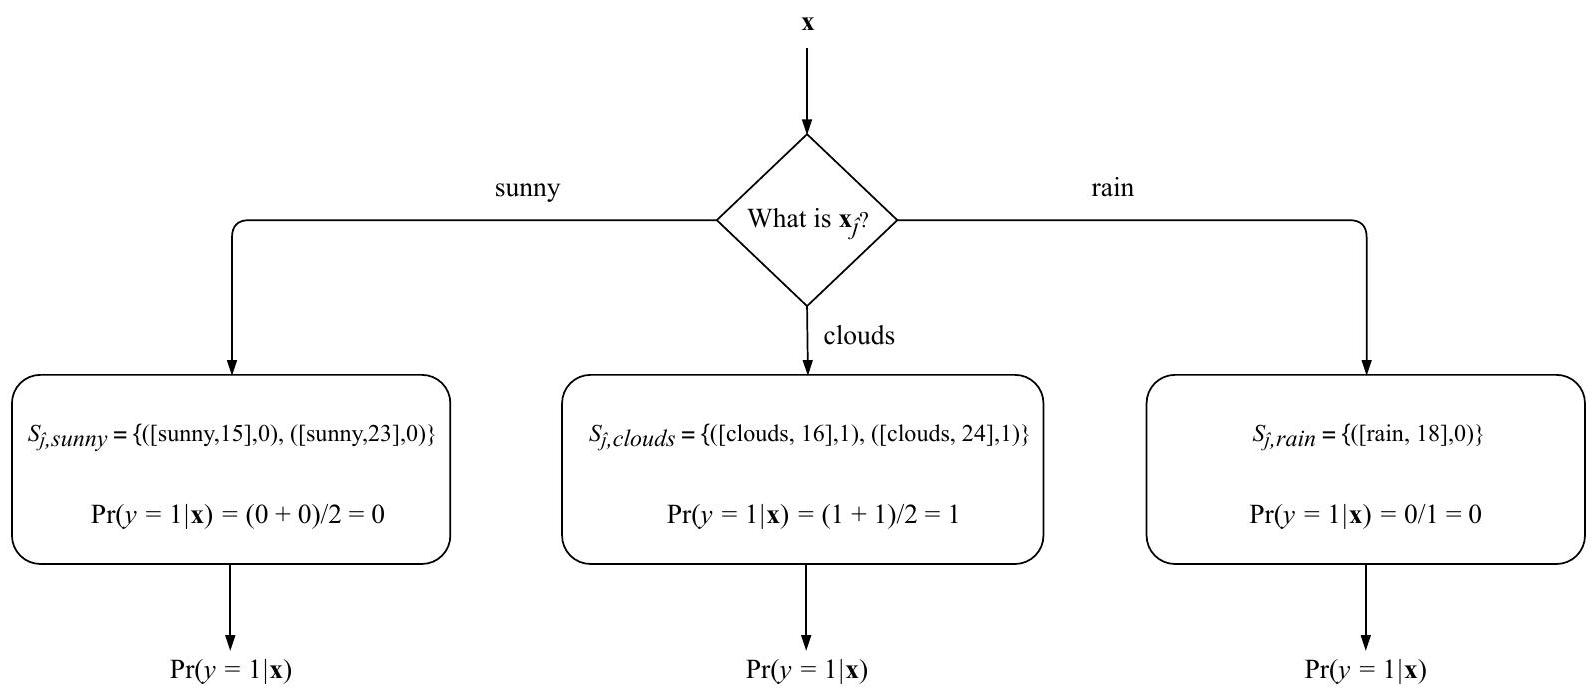
\includegraphics[width=0.7\textwidth]{imgs/algorithm_5.jpg}
			\caption{An example of a split by a categorical feature.}
		\end{figure}
		The algorithm might stop after that split, or continue by considering the second feature, "temperature", for the split in one or several of the three new leaf nodes. (We consider stopping criteria later.)
	\end{frame}
	
	\begin{frame}{Continuous Features}
		Let's now assume that feature $j$ we consider for the split is numerical like "temperature", so it has many different values (usually, much more than a categorical feature might have). 
		\begin{itemize}
			\item We want to evaluate the information gain of splitting our current leaf node by this numerical feature.
		\end{itemize}
		In C4.5, in order to deal with numerical features, the values of feature $j$ we consider for the split (for all examples in set $\mathcal{S}$ ) are sorted first.
	\end{frame}
	
	\begin{frame}
		The possible splits are shown as vertical red lines. 
		\begin{itemize}
			\item Notice, that splits are binary and only considered in areas of the sorted feature values, in which the label changes.
			\item It can be shown that splitting in the areas where the label doesn't change will not result in an improvement in the information gain.
		\end{itemize}
		 Splitting only in selected areas significantly reduces the amount of computation needed to validate each possible split.
		 \begin{figure}
		 	\centering
		 	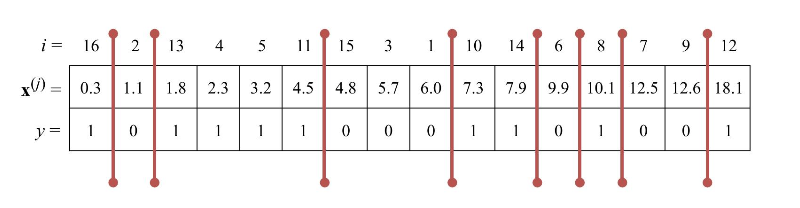
\includegraphics[width=\textwidth]{imgs/algorithm_6.png}
		 \end{figure}
	\end{frame}
	
	\begin{frame}
		One possible split is considered. Then feature $j$ is considered categorical with two values: "less than or equal to 4.5 " (the blue part) and "greater than 4.5 " (the green part).
		\begin{figure}
			\centering
			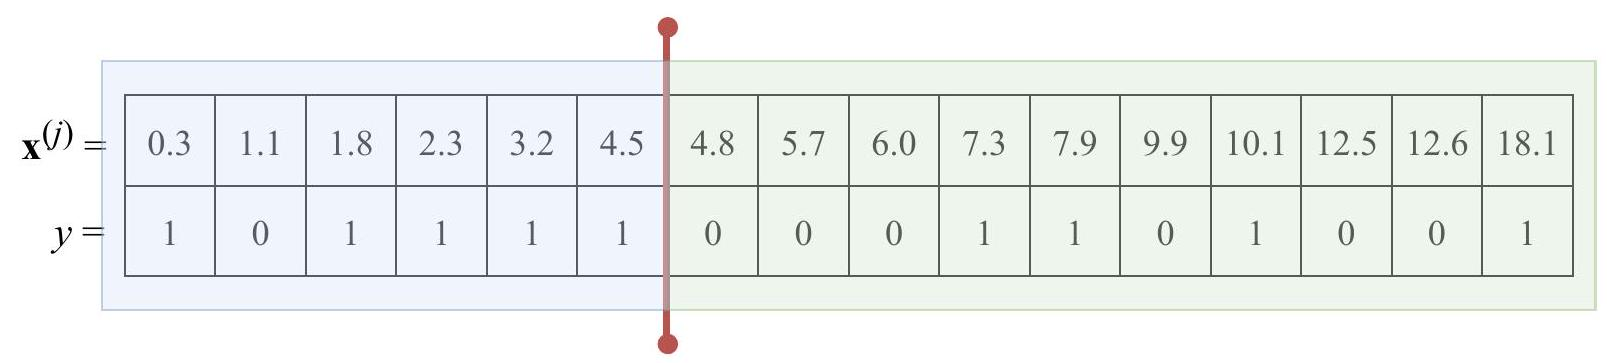
\includegraphics[width=\textwidth]{imgs/algorithm_7.jpg}
		\end{figure}
	\end{frame}
	
	\begin{frame}{Deal with Missing Values 1}
		Contrary to ID3, C4.5 can deal with missing values. The idea is quite simple. Assume that we made a split for feature $j=3$ as shown in previous figure. Then the current leaf node is split into two nodes.
		\begin{figure}
			\centering
			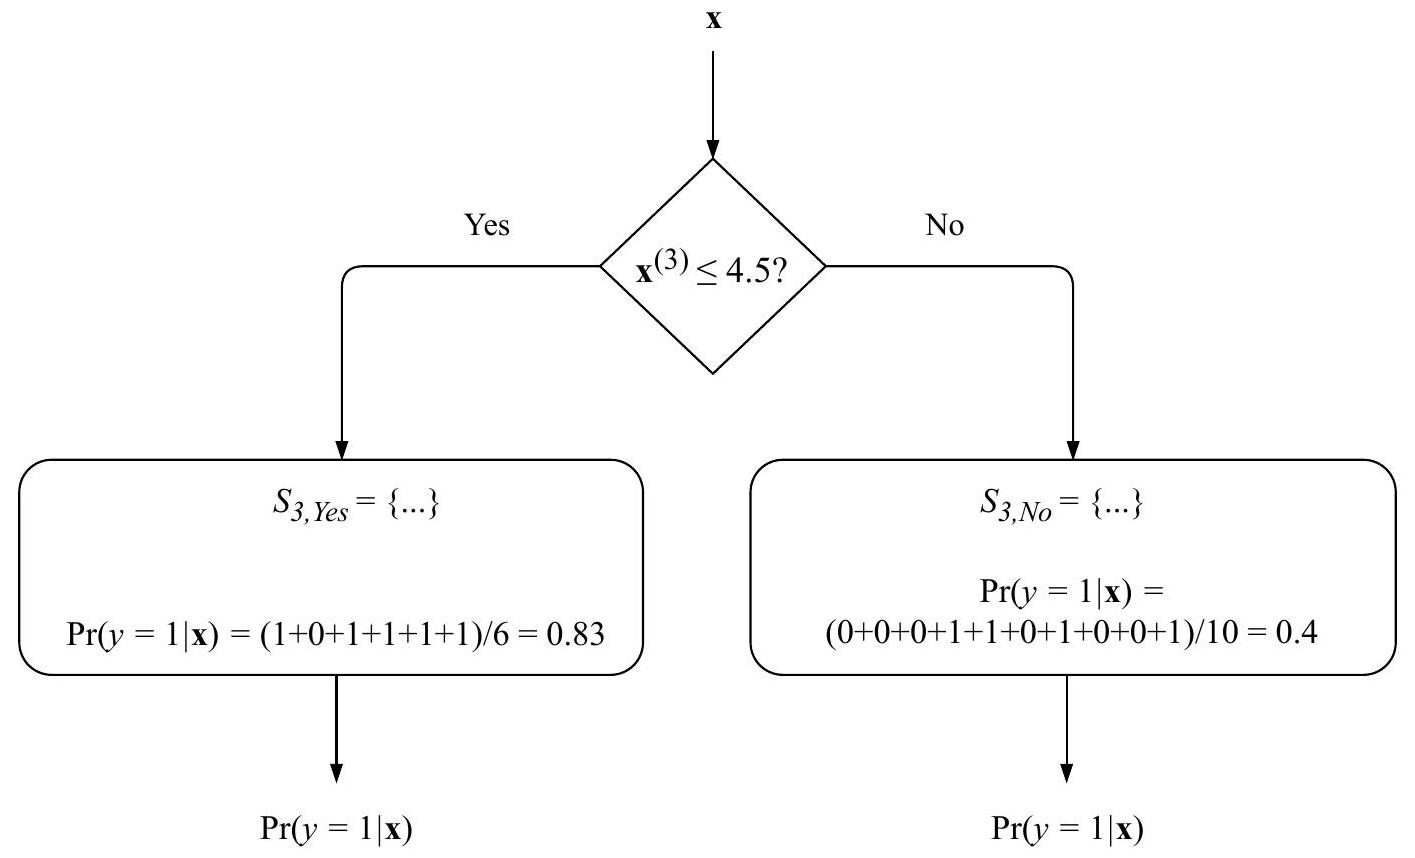
\includegraphics[width=0.7\textwidth]{imgs/algorithm_8.jpg}
			\caption{An decision node for a numerical feature.}
		\end{figure}
	\end{frame}
	\begin{frame}{Deal with Missing Values 2}
		If, in the input example $\mathbf{x}$, the value of feature $j=3$ is absent then the prediction is made in two leaf nodes at once. 
		\begin{itemize}
			\item In the left leaf node, $y=1$ with probability 0.83 ; in the right leaf node, $y=1$ with probability 0.4 ; the final prediction is $y=1$ with probability $0.83 \cdot \frac{6}{16}+0.4 \cdot \frac{10}{16}=0.5625$.
		\end{itemize}
		 If the decision threshold is 0.5 then the prediction will be $y=1$.
	\end{frame}
	
	\begin{frame}{Example: Deal with Missing Values}
		\framesubtitle{Dataset Overview}
		
		Consider a dataset predicting customer subscription to a new product:
		
		\begin{table}[h]
			\centering
			\begin{tabular}{cccc}
				\toprule
				Age & Income & Previous Subscription & Will Subscribe? \\
				\midrule
				25  & High   & Yes                   & No              \\
				40  & ?      & No                    & Yes             \\
				35  & Low    & Yes                   & Yes             \\
				30  & ?      & Yes                   & No              \\
				45  & Medium & No                    & Yes             \\
				\bottomrule
			\end{tabular}
		\end{table}
		\small{Note: '?' indicates missing values in the 'Income' feature.}
	\end{frame}
	
	\begin{frame}
		\frametitle{Decision Tree Example: Training Phase}
		\framesubtitle{Building the Tree}
		
		\begin{itemize}
			\item `Income' is chosen to split, with values `Low', `Medium', `High'.
			\item Examples with missing 'Income' are proportionally distributed:
			\begin{itemize}
				\item 50\% of 'High'/'Medium' income subscribe.
				\item 75\% of 'Low' income subscribe.
			\end{itemize}
			\item Missing income data is assigned based on these proportions.
		\end{itemize}
	\end{frame}
	\begin{frame}
		\frametitle{Decision Tree Example: Prediction Phase}
		\framesubtitle{New Customer Prediction}
		
		New customer data: Age = 32, Income = ?, Previous Subscription = Yes.
		
		\begin{itemize}
			\item At the `Income' node, the decision tree predicts using all child nodes.
			\item Predictions are combined, weighted by training phase proportions.
		\end{itemize}
	\end{frame}
	\begin{frame}
		\frametitle{Decision Tree Example: Final Prediction Calculation}
		\framesubtitle{Combining Predictions}
		
		\begin{itemize}
			\item 'Low' income node predicts 'Yes' (75\% probability).
			\item 'Medium'/'High' income nodes predict 'Yes' (50\% probability).
			\item Final prediction: \( (75\% \times 50\%) + (50\% \times 50\%) = 62.5\% \)
			\item If the threshold is 60\%, prediction for the new customer is 'Yes'.
		\end{itemize}
	\end{frame}
	
	\begin{frame}
		The C4.5 algorithm stops in some leaf node (decides not to split it) in one of the following cases:
		
		\begin{itemize}
			\item All the examples in the leaf node belong to the same class.
			\item None of the features provide any information gain.
		\end{itemize}
		You could also add additional stopping criteria and use them as hyperparameters. For example, you can decide that the algorithm will stop in a leaf node if:
		\begin{itemize}
			\item The number of examples in this leaf node is below a certain threshold.
			\item The tree is already deep enough.
		\end{itemize}
	\end{frame}
	
	\begin{frame}
		We will go over some of the key concepts on this slides in the upcoming sessions:
		\begin{itemize}
			\item One important feature of C4.5 that differs it from ID3 is that in the former there is a built-in overfitting prevention mechanism. Once the tree is built, C4.5 replaces some branches (also called \textbf{subtrees}) by leaf nodes. Doing that reduces \textbf{variance} (but inevitably increases \textbf{bias})
			\item One possible way to decide whether to keep a subtree or replace it with a leaf is to apply the tree to the examples from the validation set and measure the error made in different leaves. If the weighted sum of errors made in the leaves of some branch is higher than the error that would have been made should the tree stop one level earlier, then the branch is replaced by the leaf.
		\end{itemize}
	\end{frame}
	
	\begin{frame}
		\begin{center}
			\Huge Questions?
		\end{center}
	\end{frame}
\end{document}